\documentclass[letterpaper]{article}
\usepackage{natbib,alifexi}
<<<<<<< HEAD
\usepackage{float}
\usepackage[labelfont=bf]{caption}
\usepackage{textcomp}
=======
>>>>>>> f66aa371c92b81b2680e5db9b44ccb65c0942d5e

\title{Project Computational Game Theory\\Evolution of All-or-None Strategies in Repeated Public Goods Dilemmas}
\author{Ruben Vereecken, Yoni Pervolarakis \and Laurens Hernalsteen \\
\mbox{}\\Vrije Universiteit Brussel \\Pleinlaan 2, \\B-1050 Brussels, BELGIUM\\
{\texttt{\{rvereeck,ypervola,lhernals\}@vub.ac.be}}}


\begin{document}
\maketitle

\begin{abstract}
<<<<<<< HEAD
Engaging in repeated group interactions such as  \textit{Public Good Games}  (\textbf{PGG}), groups of individuals may contribute to a
common pool and subsequently share their resources. In this
paper we will recreate the research and results from the paper
\textit{Evolution of All-Or-None Strategies in Repeated Public Goods Dilemmas}  \citep{project}. Studying evolutionary dynamics, many strategies have emerged where individuals behave on what they observed in the previous round. One such strategy is the simple \textit{All-Or-None} \textbf{(AON)} strategy, which consists of cooperating only after an unanimous group choice. In this paper, we test the AON strategy, along with a variant of our own (NQAON) where the group choice can deviate a small percentage from being unanimous. We explore the effect of changing the parameters of both strategies and examine their robustness. We find that \textit{Not Quite All-Or-Nothing} \textbf{(NQAON)} outperforms AON in areas where it tends to fall victim to its own simplicity.
=======
Engaging in repeated group interactions such as \textit{Public Good Games}  (\textbf{PGG}), groups of individuals may contribute to a common pool and subsequently share their resources. In this paper we will recreate the research and results from the paper  \textit{Evolution of All-Or-None Strategies in Repeated Public Goods Dilemmas}  \citep{project}. Studying evolutionary dynamics, where individuals behave on what they observed in the previous round, the simple \textit{All-Or-None} \textbf{(AON)} strategy  will emerge. AON consists of cooperating only after an unanimous group choice. We prove the robustness of this strategy by using different group sizes and error rates
\textit{\textbf{Short summary of results....}}
>>>>>>> f66aa371c92b81b2680e5db9b44ccb65c0942d5e


\end{abstract}

\section{Introduction}
When studying \textit{Public Good Games}  (\textbf{PGG}), such as \textit{N-person Prisoner's Dilemma}  (\textbf{NPD}), social dilemma's arise where self-serving behavior is worse than collective behavior \citep{kollock1998social}. These problems can be found in economics as well in biology.
Without additional mechanisms such as risk of future loss \citep{santos2011risk}, institutions who deal with free-riders who choose not to contribute \citep{vasconcelos2013bottom,sigmund2010social}, thresholds that must be surpassed before collecting action can be successful \citep{pacheco2011evolutionary}, a network of interactions or social diversity \citep{wang2013interdependent,santos2008social}, punishment \citep{fehr2002altruistic,brandt2006punishing} or voluntary participation \citep{hauert2002volunteering} there is a possibility that populations will fall into a tragedy of the commons \citep{hardin1968tragedy}.
<<<<<<< HEAD
Collective action problems often involve repeated actions between individuals of the same group \citep{boyd1988evolution}. Real life examples can be found in world leaders trying to cooperate in changing the climate problems \citep{milinski2008collective,barrett2012climate}, the monetary crisis \citep{jacquet2001economic} and even in anarchies \citep{axelrod1985achieving}. This leads to the question whether direct reciprocity can escape the tragedy of the commons. If we subdivide this question, it is difficult to find to whom one should reciprocate in repeated N-player interactions. Direct reciprocity has been generalized for PGG where individuals of group size N only cooperate if there are at least M $(0<=M<=N)$ cooperators in the previous round \citep{van2012emergence,kurokawa2009emergence}. Such generalized reciprocators provide a generalization of the \textit{Tit For Tat}  (\textbf{TFT}) strategy, but they constitute a small set of all individual strategies.
In this research different strategies will be explored, where individuals may adopt a different strategy when playing PGG on the condition that their actions are based on the behavior of the group in the previous round.
The goal of this project is to research the AON strategy as proposed in the Evolution of All-Or-None Strategies in Repeated Public
Goods Dilemmas \citep{project} paper. Not-Quite-All-Or-Nothing (\textbf{NQOAN}), a variant of the All-Or-None strategy where players cooperate if a fixed percentage of players cooperate or defect, will also be explored and subjected to the same tests.

\section{Methods}
Let us consider a finite and will-mixed population $Z$, with only cooperators and defectors, who randomly form groups of size $N$ and play the repeated version of NPD. In every round individuals can either cooperate (\textbf{C}) by contributing an amount $c$ to a public pool or defect (\textbf{D}). The sum of contributions of a group per round is multiplied by an enhancement factor $F$ and will become a public good to the group. This will be equally divided amongst  the $N$ individuals. In each round defectors will receive a payoff of $\pi_{D}= \frac{kFc}{N}$  and cooperators will receive $\pi_{C}=\pi_{D}-c$ where $k$ is the number of cooperators in that round. In this model PGG will have an undetermined amount of rounds, where at the end of every round another round might take place with probability $w$. This leads to an average amount of rounds, denoted as $m$, where $m= (1-w)^{-1}$. Individuals decide in each round, except the first round, to cooperate or not based on the total amount of contributions in the previous round.
=======
Collective action problems often involve in repeated actions between individuals of the same group \citep{boyd1988evolution}. Real life examples can be found in world leaders trying to cooperate in changing the climate problems \citep{milinski2008collective,barrett2012climate}, the monetary crisis \citep{jacquet2001economic} and even in anarchies \citep{axelrod1985achieving}. This leads to the question whether direct reciprocity can escape the tragedy of the commons. If we subdivide this question, it is difficult to find to whom one should reciprocate in repeated N-player interactions. Direct reciprocity has been generalized for (\textbf{PGG}) where individuals of group size N only cooperate if there are at least M $(0<=M<=N)$ cooperators in the previous round \citep{van2012emergence,kurokawa2009emergence}. Generalized reciprocators provide a generalization of the \textit{Tit For Tat}  (\textbf{TFT}) strategy, but they constitute a small set of all individual strategies.
In this research exploration of different strategies will be explored, where individuals may adopt a different strategy when playing PGG on the condition that their actions are based on the behavior of the group in the previous round.
\textit{\textbf{more??}}

\section{Methods}
Let us consider a finite and will-mixed population $Z$, with only cooperators and defectors, who randomly form groups of size $N$ and play the repeated version of \textbf{NPD}. In every round individuals can either cooperate (\textbf{C}) by contributing an amount $c$ to a public pool or defect (\textbf{D}). The sum contributions of a group are per round are multiplied by an enhancement factor $F$ and will become a public good to the group. This will equally be divided amongst  the $N$ individuals. In each round defectors will achieve a payoff of $\pi_{D}= \frac{kFc}{N}$  and cooperators will achieve $\pi_{C}=\pi_{D}-c$ where $k$ is the number of cooperation in that round. In this model \textbf{PGG} will have an undetermined amount of rounds, where at the end of every round another round might take place with probability $w$. This leads to an average amount of rounds, denoted as $m$, where $m= (1-w)^{-1}$. Individuals decide in each round, except the first round, to cooperate or not based on the total amount of contributions in the previous round.
\textit{\textbf{...bitshizzle...}}
>>>>>>> f66aa371c92b81b2680e5db9b44ccb65c0942d5e
The Fermi update rule \citep{traulsen2006stochastic,grujic2014comparative} is used each round to revise the strategies of the individuals.
In each round a random individual $A$ will be chosen, with its strategy $S_{A}$ and fitness $f_{_f{A}}$. The fitness of a strategy is the average payoff over all rounds for that strategy. Individual $A$ can change its strategy through $i)$ mutating with probability $\mu$ or $ii)$ by imitating a random individual $B$ with probability $(1-\mu)(1+exp[-\beta(f_{_S{A}}-f_{_S{B}})])^{-1}$, where $\beta$ is the intensity of selection.
In each round after choosing to cooperate or defect, an individual may choose the opposite behavior with a probability of $\epsilon$.
Additionally, the AON strategy will be examined with different enhancement factors to test if there is a difference, different groups sizes and finally tested against the NQAON strategy where a small percentage of the individuals can deviate from being unanimous.


<<<<<<< HEAD

\section{Results and discussion}
If we denote $\eta$ as the behavioral fraction of cooperation we get the graph depicted in Fig.~\ref{fig1}. Not every simulation will end in the same round, because of the probability of $w$. We show the mean of all simulations up to the round that at least a quarter of the simulations can reach for representativity.
\vspace{5 mm}
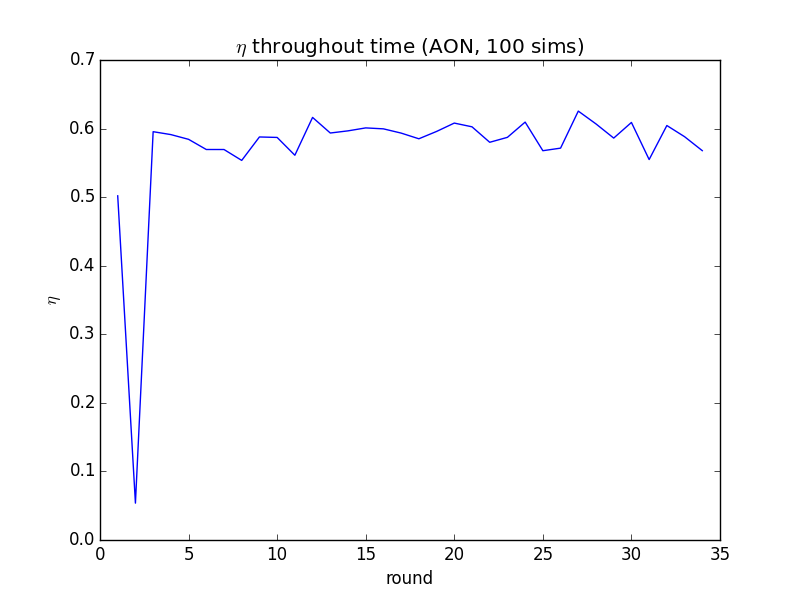
\includegraphics[width=3.6in,angle=0]{img/cfraction_aon.png}
\captionof{figure}{Cooperation fraction throughout time (100 sims). Where $Z=100$, $N=10$, $F=8$, $c= 2$, $\beta=1$, $\epsilon=0.05$, $\mu=0.001$ and the initial \textbf{$\eta$} $= 0.5$}
\label{fig1}
\vspace{5 mm}

As can be seen in Fig.~\ref{fig1}, in the first round almost all simulations will go near $0.05$. This is due to the fact that in the first round all choices are generated randomly and are therefore strongly unanimous, resulting in a second round of large-scale defection. After this we get an average of $0.6$ because of choice changes as a result of the $\epsilon$  value.
In Fig.~\ref{fig2} we will test the robustness of the AON strategy. Note that all configuration parameters will be the same as in Fig.~\ref{fig1} except where reported otherwise. As can be seen when $\epsilon$ is very low we get a high behavioral fraction as opposed to a high $\epsilon$. This result is to be expected, as an $\epsilon$ nearing zero stands for a group of AON players that almost never behave unexpectedly and will converge towards cooperating nearly every time.

\vspace{5 mm}
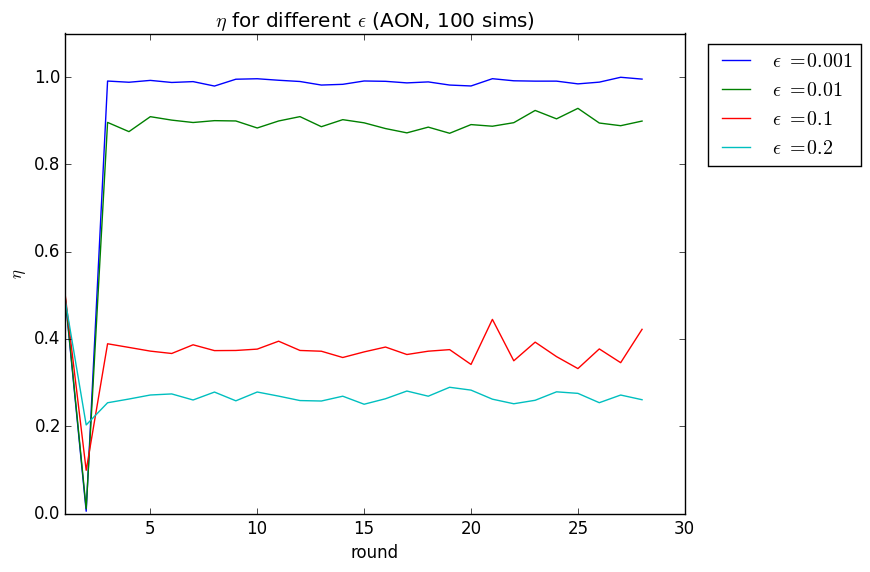
\includegraphics[width=3.6in,angle=0]{img/cfraction_epsilon_aon.png}
\captionof{figure}{Cooperation fraction throughout time (100 sims) with different $\epsilon$.}
\label{fig2}
\vspace{5 mm}

=======

\section{Results}

>>>>>>> f66aa371c92b81b2680e5db9b44ccb65c0942d5e

\begin{figure}[!htb]
\begin{center}
\includegraphics[width=3in,angle=0]{img/CooperationFrac.png}
\caption{Cooperation fraction throughout time (100 sims).}
\label{fig1}
\end{center}
\end{figure}

% In Fig.~\ref{fig2}

<<<<<<< HEAD

As can be seen on Fig.~\ref{fig3}, the higher the enhancement factor $F$ is, the higher the mean will be, which is a logical consequence. It is also shown that in these simulations, the strategy has a negative return if $F<2$, meaning that pooled resources need to be at least doubled by an external entity for the strategy to be viable.


\vspace{5 mm}
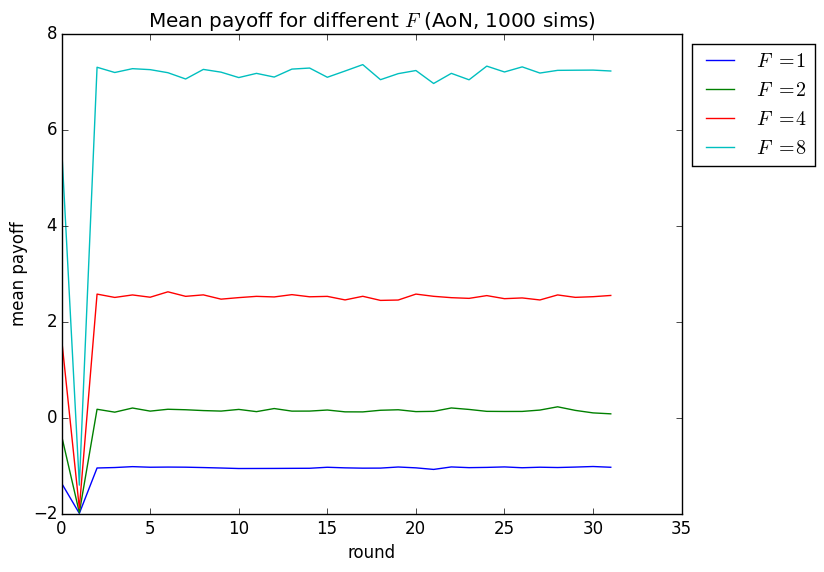
\includegraphics[width=3.6in,angle=0]{img/meanpayoff_F_aon.png}
\captionof{figure}{Mean payoff for different $F$}
\label{fig3}
\vspace{5 mm}

Fig.~\ref{fig4} shows that there is no meaningful difference for varying values of $F$. This is an intuitive result, seeing as none of the players using the AON strategy make use of the previous or expected payoff to choose C or D. Note that the payoff for a population with only cooperators would be a constant $c(F-1)$.


\vspace{5 mm}
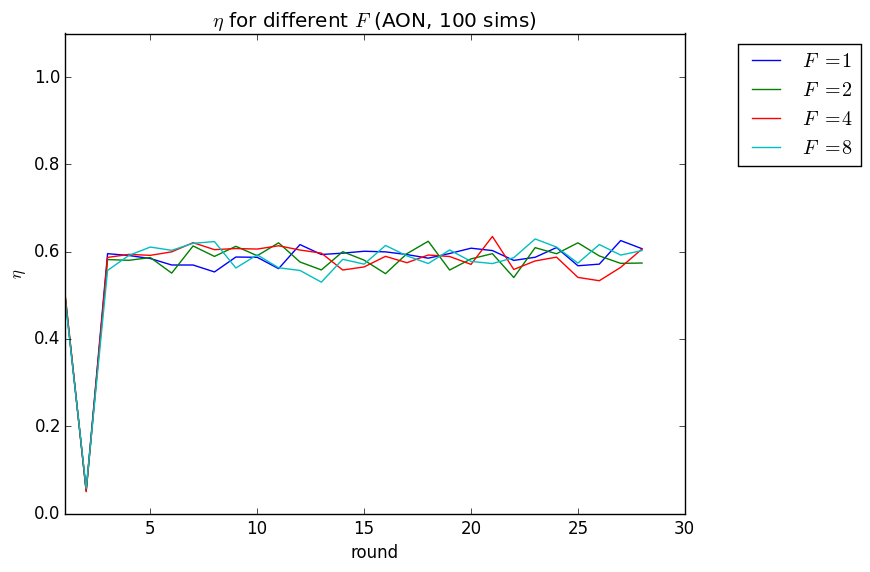
\includegraphics[width=3.6in,angle=0]{img/cfraction_F_aon.png}
\captionof{figure}{$\eta$ for different enhancement factor $F$}
\label{fig4}
\vspace{5 mm}


Fig. ~\ref{fig5} shows us that every player has a small probability of changing its choice, the probability that one or more players will defect when the rest cooperates or vice versa, rises linearly with the number of players. As only one player needs to behave differently from the rest to offset the collective choice and effect a situation where every AON player defects, it stands to reason that the more players there are, the more rounds will result in defection.
\vspace{5 mm}


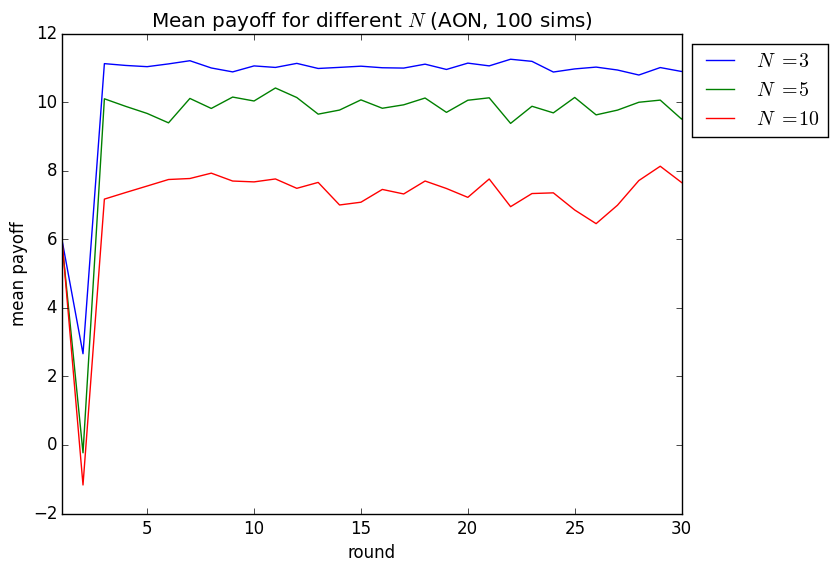
\includegraphics[width=3.6in,angle=0]{img/meanpayoff_N_aon.png}
\captionof{figure}{Mean payoff for different $N$}
\label{fig5}
\vspace{5 mm}


To test the viability of AON we mixed its population with \textbf{AllC} and \textbf{AllD} (unconditional cooperators and defectors respectively). The results of these experiments can be witnessed in Figures ~\ref{fig6} and ~\ref{fig7}. Every line denotes the cooperation fraction for a different starting fraction of AON players. 
\includegraphics[width=3.6in,angle=0]{img/cfraction_AONAllCfractions_aon.png}
\captionof{figure}{$\eta$ for different AON/AIIC}
\label{fig6}
\vspace{5 mm}

\includegraphics[width=3.6in,angle=0]{img/cfraction_AONAllDfractions_aon.png}
\captionof{figure}{$\eta$ for different AON/AIID} 
\label{fig7}
\vspace{5 mm}
As can be seen, the populations quickly become fairly stagnant even though the mix with AllD tends to fluctuate more towards the beginning. Sadly, due to our model, a change in strategy is only allowed once per round and then only for one random individual. We expect more violent changes in population distribution would otherwise have occurred.
Let us now inspect the impact of starting conditions on the course of the game.

Fig. ~\ref{fig6} shows a positive correlation between AllC players and $\eta$. Why though do AON players seem to defect en masse when AllC players are present? This is because of the population\textquotesingle s inability to come to an unanimous decision. In pure AON populations we observe a round of mass defection, followed by cooperation. This mass defection has now become impossible by the influence of the AllC immigrants, rendering the AON players unable to ever cooperate. Let $\alpha$ be the fraction of AON players, then the average fraction of cooperators each round lies around $1-\alpha$. This behavior works out positively for the AON player in situations with large fractions of AllC players, depending on the multiplication factor, because these AON players effectively cheat the system of AllC players. We have also confirmed that there is a slight decline in the population of AON players where there are not too many AllC players to begin with (in these cases the AON players make more profit), meaning AON players actually migrate to becoming AllC. Once again this effect is not immensely present due to our model.

For AllD, we observe that the more AllD players the game starts with, the less cooperation there is. It is clearly shown that AON is unable to sustain itself when unconditional defectors are present. Every time the AON players collectively choose to cooperate, the fraction of cooperation will near $\alpha$. But every following round, that fraction will near zero because the presence of the AllD players will make those AON players defect. This behavior then is flipped again the next round when the AON players react to the full defection by again choosing to collectively cooperate. Due to this alternating behavior, the average of AON players when mixed with AllD players will approach $\alpha/2$. The maximum $\eta$ is therefore capped at $0.5$. This effect is further worsened by errors. This phenomenon can be seen as a sense of self-preservation where a player that gets cheated on too often cheats itself to avoid being duped.


\vspace{5 mm}
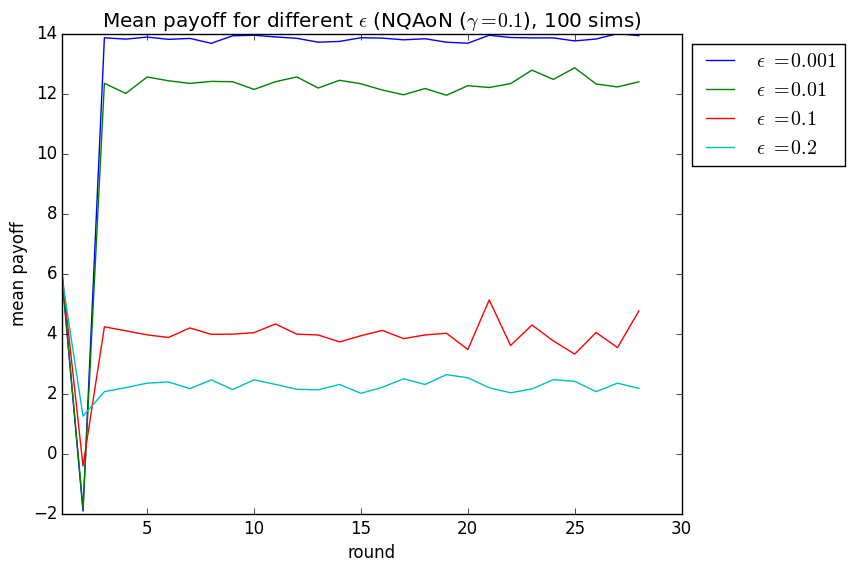
\includegraphics[width=3.6in,angle=0]{img/meanpayoff_epsilon_nqaongamma01.png}
\captionof{figure} {Mean payoff (NQOAN) with $\epsilon$ and $\gamma=0.01$}
\label{fig8}
\vspace{5 mm}

As can be seen from Fig. ~\ref{fig8} and Fig. ~\ref{fig9}, the mean payoff for NQAON lies higher than that of AON for every value of $\epsilon$ and $\gamma=0.1$ and $\gamma=0.2$. The $\gamma$ parameter represents the fraction of the group that is allowed to deviate from the popular decision. This happens because NQAON allows for a certain fraction ($\gamma$) of players to deviate from the overall choice, rather than requiring a unanimous choice. These results will obviously become worse if $\gamma$ becomes too large, because then the NQAON players would encourage others to defect. We suspect there to be a value for $\gamma$ where the mean payoff NQAON and that of AON become the same.


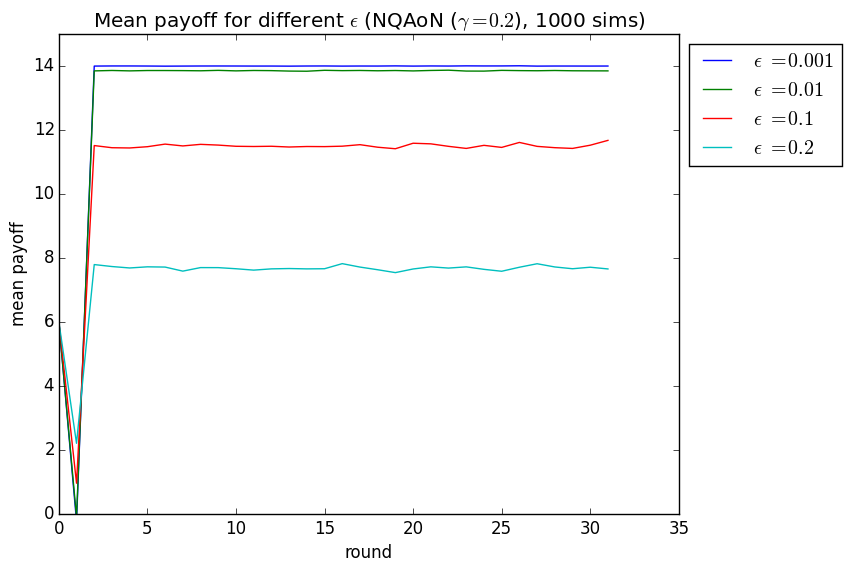
\includegraphics[width=3.6in,angle=0]{img/meanpayoff_epsilon_nqaongamma02.png}
\captionof{figure} {NQAON fraction with $\epsilon$ and $\gamma=0.02$}
\label{fig9}
\vspace{3 mm}

\section{Conclusion}

To conclude our research, we see that AON is not as powerful as initially thought. The reason for this is that AON doesn't cope well with increasing error rates. There are occasions where it performs well (in competition with a large AllC fraction for example), because then it can profit from defecting. However, we know this is an artificial example that would not exist in the real world and that the AON strategy then promotes defection over cooperation, eventually resulting in a change from AON strategy to an AllD strategy. The AON strategy was also shown to not be viable when $F<2$. Although some results for higher values of $F$ look promising, real life examples wherein an external contributor multiplies pooled resources out of generosity seem unrealistic.
The NQAON was shown to behave more predictable because it is less influenced by small values. We still see that NQAON does not promote cooperation when the fraction of unconditional cooperators exceeds $\gamma$.
NQAON with $\gamma = 0.2$ was shown to have better results than where $\gamma=0.1$. There obviously is a limit to the value of $\gamma$ where the fraction of contrary choices should no longer be ignored. It might be interesting to see results of NQAON with $\gamma$ as a continuous parameter in various situations. It could also prove insightful to research situations in which both AON and NQAON are present.
Both AON and NQAON are rather artificial and would not come intuitively to the human mind without clearly communicating the strategies as a group beforehand. Therefore, it could prove insightful to pitch the AON/NQAON players in a group with real people, to see how they would react to (or exploit) the AON/NQAON players.

\section{Materials \& Techniques}
The code for this research is available as an iPython Notebook at https://github.com/rubenvereecken/allornone. It contains several functions that allow completely automated parameter exploration and plotting of our models, including easily introducing new behavioral strategies. All supplied material is available under the MIT license. 

\section{Acknowledgments}
We want to show our gratitude to Fl\'{a}vio L. Pinheiro for responding to our questions and helping us.

=======
\section{Discussion}
Something something

\section{Acknowledgments}
>>>>>>> f66aa371c92b81b2680e5db9b44ccb65c0942d5e

Help from Fl\'{a}vio L. Pinheiro....


\footnotesize
\bibliographystyle{apalike}
\bibliography{biblio}


\end{document}
